%%%%%%%%%%%%%%%%%%%%%%%%%%%%% Define Article %%%%%%%%%%%%%%%%%%%%%%%%%%%%%%%%%%
\documentclass{article}
%%%%%%%%%%%%%%%%%%%%%%%%%%%%%%%%%%%%%%%%%%%%%%%%%%%%%%%%%%%%%%%%%%%%%%%%%%%%%%%

%%%%%%%%%%%%%%%%%%%%%%%%%%%%% Using Packages %%%%%%%%%%%%%%%%%%%%%%%%%%%%%%%%%%
\usepackage{geometry}
\usepackage{graphicx}
\usepackage{amssymb}
\usepackage{amsmath}
\usepackage{amsthm}
\usepackage{empheq}
\usepackage{mdframed}
\usepackage{booktabs}
\usepackage{lipsum}
\usepackage{graphicx}
\usepackage{color}
\usepackage{psfrag}
\usepackage{pgfplots}
\usepackage{bm}
%%%%%%%%%%%%%%%%%%%%%%%%%%%%%%%%%%%%%%%%%%%%%%%%%%%%%%%%%%%%%%%%%%%%%%%%%%%%%%%

% Other Settings

%%%%%%%%%%%%%%%%%%%%%%%%%% Page Setting %%%%%%%%%%%%%%%%%%%%%%%%%%%%%%%%%%%%%%%
\geometry{a4paper}

%%%%%%%%%%%%%%%%%%%%%%%%%% Define some useful colors %%%%%%%%%%%%%%%%%%%%%%%%%%
\definecolor{ocre}{RGB}{243,102,25}
\definecolor{mygray}{RGB}{243,243,244}
\definecolor{deepGreen}{RGB}{26,111,0}
\definecolor{shallowGreen}{RGB}{235,255,255}
\definecolor{deepBlue}{RGB}{61,124,222}
\definecolor{shallowBlue}{RGB}{235,249,255}
%%%%%%%%%%%%%%%%%%%%%%%%%%%%%%%%%%%%%%%%%%%%%%%%%%%%%%%%%%%%%%%%%%%%%%%%%%%%%%%

%%%%%%%%%%%%%%%%%%%%%%%%%% Define an orangebox command %%%%%%%%%%%%%%%%%%%%%%%%
\newcommand\orangebox[1]{\fcolorbox{ocre}{mygray}{\hspace{1em}#1\hspace{1em}}}
%%%%%%%%%%%%%%%%%%%%%%%%%%%%%%%%%%%%%%%%%%%%%%%%%%%%%%%%%%%%%%%%%%%%%%%%%%%%%%%

%%%%%%%%%%%%%%%%%%%%%%%%%%%% English Environments %%%%%%%%%%%%%%%%%%%%%%%%%%%%%
\newtheoremstyle{mytheoremstyle}{3pt}{3pt}{\normalfont}{0cm}{\rmfamily\bfseries}{}{1em}{{\color{black}\thmname{#1}~\thmnumber{#2}}\thmnote{\,--\,#3}}
\newtheoremstyle{myproblemstyle}{3pt}{3pt}{\normalfont}{0cm}{\rmfamily\bfseries}{}{1em}{{\color{black}\thmname{#1}~\thmnumber{#2}}\thmnote{\,--\,#3}}
\theoremstyle{mytheoremstyle}
\newmdtheoremenv[linewidth=1pt,backgroundcolor=shallowGreen,linecolor=deepGreen,leftmargin=0pt,innerleftmargin=20pt,innerrightmargin=20pt,]{theorem}{Theorem}[section]
\theoremstyle{mytheoremstyle}
\newmdtheoremenv[linewidth=1pt,backgroundcolor=shallowBlue,linecolor=deepBlue,leftmargin=0pt,innerleftmargin=20pt,innerrightmargin=20pt,]{definition}{Definition}[section]
\theoremstyle{myproblemstyle}
\newmdtheoremenv[linecolor=black,leftmargin=0pt,innerleftmargin=10pt,innerrightmargin=10pt,]{problem}{Problem}[section]
%%%%%%%%%%%%%%%%%%%%%%%%%%%%%%%%%%%%%%%%%%%%%%%%%%%%%%%%%%%%%%%%%%%%%%%%%%%%%%%

%%%%%%%%%%%%%%%%%%%%%%%%%%%%%%% Plotting Settings %%%%%%%%%%%%%%%%%%%%%%%%%%%%%
\usepgfplotslibrary{colorbrewer}
\pgfplotsset{width=8cm,compat=1.9}
%%%%%%%%%%%%%%%%%%%%%%%%%%%%%%%%%%%%%%%%%%%%%%%%%%%%%%%%%%%%%%%%%%%%%%%%%%%%%%%

%%%%%%%%%%%%%%%%%%%%%%%%%%%%%%% Title & Author %%%%%%%%%%%%%%%%%%%%%%%%%%%%%%%%
\title{Rolle's Theorem, Mean Value Theorem, and Graphing}
\author{Patrick Chen}
\date{Oct 7, 2024}
%%%%%%%%%%%%%%%%%%%%%%%%%%%%%%%%%%%%%%%%%%%%%%%%%%%%%%%%%%%%%%%%%%%%%%%%%%%%%%%

\begin{document}
    \maketitle
    \section*{Rolle's theorem}
    if $f$ is continuous on the closed interval $[a,b]$, $f$ is differentiable
    on the open interval $(a,b)$, and $f(a)=f(b)$, then there is a number $c$ in
    $(a,b)$ such that $f'(c) = 0$

    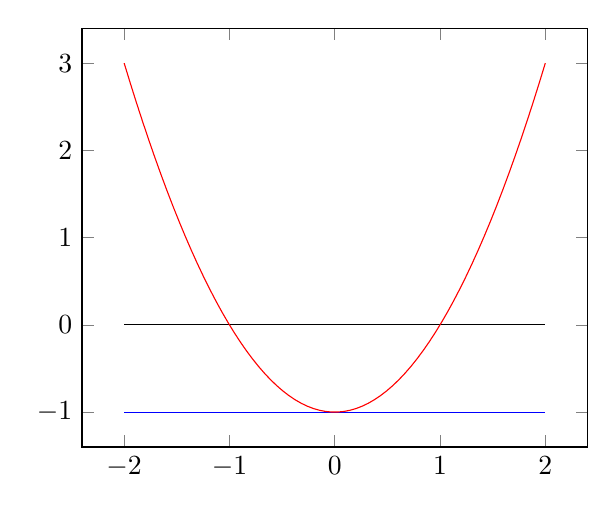
\begin{tikzpicture}
         \begin{axis}
             \addplot [
                domain=-2:2,
                samples=70,
                color=blue,
                ]
                {-1};
             \addplot [
                domain=-2:2,
                samples=70,
                color=black,
                ]
                {0};
             \addplot [
                domain=-2:2,
                samples=70,
                color=red,
                ]
                {x^2 - 1};
         \end{axis}
    \end{tikzpicture}

    This theorem fails if the function is either non-differentiable or not
    continuous.

    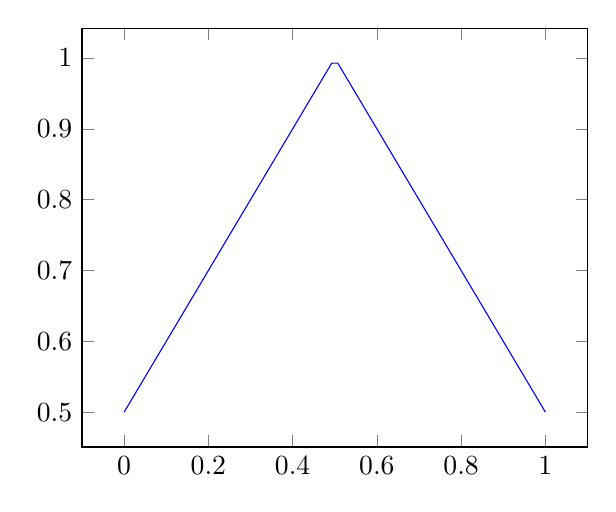
\begin{tikzpicture}
         \begin{axis}
             \addplot [
                domain=0:1,
                samples=70,
                color=blue,
                ]
                {-abs(x-0.5)+1};
         \end{axis}
    \end{tikzpicture}

    \begin{tikzpicture}
         \begin{axis}
             \addplot [
                domain=0.5:1,
                samples=70,
                color=blue,
                ]
                {0};
             \addplot [
                domain=0:0.5,
                samples=70,
                color=blue,
                ]
                {x^2};
         \end{axis}
    \end{tikzpicture}

    \subsection*{Example}
    Prove that $x^3+x-1=0$ has exactly one root.

    To do this, we must prove that the function has at least one root, then show
    that there exists no more than one root.

    \begin{align*}
        f(0) &= 0^3 +0 - 1 \\
        f(0) &= -1 \\
        f(1) &= 1^3 + 1 - 1 \\
        f(1) &= 1
    \end{align*}
    Since polynomial functions are continuous, by the intermediate value
    theorem, there must exist a root in the interval $(0,1)$.

    To prove that there does not exists two roots $x_1,x_2$, assume there are two roots.
    By Rolle's theorem, there exists a point $c$ where $f'(c)=0$. Since the
    derivative is never zero, this is a contradiction and there cannot be two
    roots.
    \begin{align*}
        f(x) = x^3 +x - 1 \\
        f'(x) = 3x^2 + 1
    \end{align*}

    \section*{Mean Value Theorem}
    For a function $f$ that is continuous on the closed interval $[a,b]$ and
    differentiable on the open interval $(a,b)$, then there is a number $c$ in
    $(a,b)$ such that $f'(c)= \frac{f(b)-f(a)}{b-a}$.

    In other words, if a function is continuous and differentiable on a
    interval, then there is a point in that interval where the slope is equal to
    the secant line formed by the two endpoints. The mean value theorem is a
    generalized version of Rolle's theorem. \\
    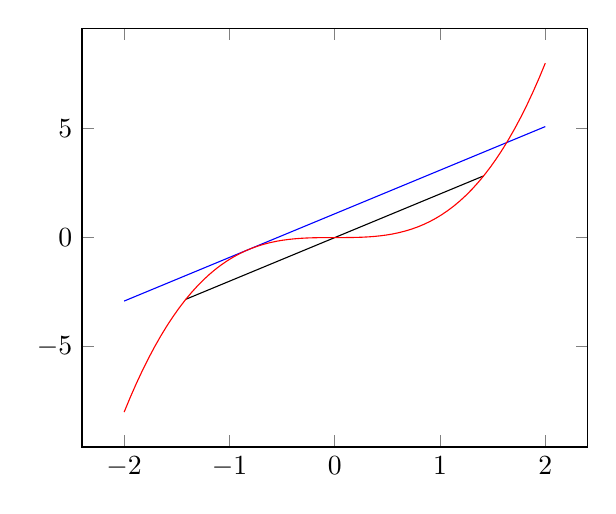
\begin{tikzpicture}
         \begin{axis}
             \addplot [
                domain=-1.414:1.414,
                samples=70,
                color=black,
                ]
                {2*x};
             \addplot [
                domain=-2:2,
                samples=70,
                color=blue,
                ]
                {2*x+1.09};
             \addplot [
                domain=-2:2,
                samples=70,
                color=red,
                ]
                {x^3};
         \end{axis}
    \end{tikzpicture}

    \subsection*{Example}
    If $f(0)=-3$ and $f'(x)\le 5$, for all x, how large can $f(2)$ possible be.
    Using the interval $[0,2]$:
    \begin{align*}
        f'(c) &= \frac{f(b)-f(a)}{b-a} \\
              &= (f(2)-3)/(2-0) \\
              &= (f(2)+3)/2 \\
        f(2)  &= 2f'(c) - 3 \\
        f(2)  &\le 2(5) - 3 \\
        f(2)  &\le 7
    \end{align*}

    \section*{Derivative information}
    \begin{itemize}
        \item if $f'(x) > 0$ on an interval, then $f$ is increasing on that
            interval
        \item if $f'(x) < 0$ on an interval, then $f$ is increasing on that
            interval
    \end{itemize}

    For a continuous function $f$ and a critical value $c$
    \begin{itemize}
        \item if $f'$ changes from positive to negative at $c$, then $f$ has
            local max at c.
        \item if $f'$ changes from negative to positive at $c$, then $f$ has
            local min at c.
        \item if $f'$ is positive to left and right of $c$, or negative to left
            and right of $c$, then $f$ has no local maximum or minimum.
    \end{itemize}

    A function $f$ is called concave upward on an interval $I$ if all tangents
    lays below the function on the interval $I$.

    \begin{itemize}
        \item If $f''(x)>0$ on an interval $I$, then the graph of $f$ is
            concave upward on $I$
        \item If $f''(x)<0$ on an interval $I$, then the graph of $f$ is
            concave downward on $I$
    \end{itemize}

    A point $(x,y)$ on a curve $y=f(x)$ is called an inflection point if $f$ is
    continuous there and the curve changes from concave up to concave down or
    from concave down to concave up at $x$. Just like the first derivative, if
    $f''(x)=0$, then there is not always a inflection point.

    \begin{itemize}
        \item If $f'(c)=0$ and $f''(c)>0$, then $f$ has a local minimum at $c$.
        \item If $f'(c)=0$ and $f''(c)<0$, then $f$ has a local maximum at $c$.
    \end{itemize}

    \subsection*{Example: Graphing}
    \begin{align*}
        f(x) = x^{2/3}(6-x)^{1/3} \\
        f'(x) = \frac{4-x}{x^{1/3}(6-x)^{2/3}} \\
        f''(x) = -\frac{8}{x^{4/3}(6-x)^{5/3}}
    \end{align*}

    \begin{align*}
        f(0) = 0 &\\
        f(x) = 0 &\Rightarrow x=0,6 \\
    \end{align*}

    $f'$ is zero when $x=4$ and $f'$ is undefined when $x=0,6$.
    \begin{center}
        \begin{tabular}[c]{l|l|l|l|l|l|l|l}
            \hline
            & $x<0$ & $x=0$ & $0<x<4$ & $x=4$ & $4<x<6$ & $x=6$ & $6<x$ \\
            \hline
            f  & + & 0   & + & + & + & 0   & - \\
            && $m=\infty$ && local max && $m=\infty$ & \\
            f' & - & DNE & + & 0 & - & DNE & - \\
            f''& - & DNE & - & - & - & DNE & + \\
            \hline
        \end{tabular}
    \end{center}

    \begin{tikzpicture}
         \begin{axis}
             \addplot [
                domain=-10:10,
                samples=70,
                color=blue,
                ]
                {(x^2)^(1/3)*sign(6-x)*(abs(6-x))^(1/3)};
         \end{axis}
    \end{tikzpicture}
\end{document}
